\documentclass[11pt]{article}
%\documentclass{book}
\usepackage[utf8]{inputenc}
\usepackage[T1]{fontenc}
\usepackage[french]{babel}
\usepackage[top=1.8cm, bottom=1.8cm, left=1.8cm, right=1.8cm]{geometry}
\usepackage[linktocpage,colorlinks=false]{hyperref}
\usepackage{graphicx}
\usepackage{epsfig}
\usepackage{amssymb}
\usepackage{amsmath}
\usepackage{array}
\usepackage{subfig}
\usepackage{multicol}
\usepackage{caption}
\usepackage{listings}
\usepackage{algorithm}
\usepackage{algorithmic}
\hypersetup{
    colorlinks=true,
    breaklinks=true,
    urlcolor=red,
}
\parskip=5pt

\title{\huge{\textbf Spécifications}}
\author{AYOUB Pierre, BASKEVITCH Claire, BESSAC Tristan, \\
CAUMES Clément, DELAUNAY Damien, DOUDOUH Yassin}
\date{Mercredi 18 Avril 2018}

\begin{document}

\maketitle
\vspace{20em}
\begin{center}
\includegraphics{pictures/Application.png}\end{center}
\newpage

\tableofcontents

\newpage

\section{Introduction}

En réalisant le cahier des charges concernant l'application StegX, 
l'analyse des contraintes et des besoins du client nous amène à rédiger 
les spécifications. 

Le logiciel StegX pourra proposer de cacher des données dans des fichiers 
dont le format est pris en charge par l'application. De plus, un utilisateur 
pourra extraire les données cachées d'un fichier qu'on considère déjà comme 
hôte. StegX prendra en charge les trois algorithmes de stéganographie suivants : 
EOF, LSB et MetaData. 

Avec l'analyse des fonctionnalités de l'application, nous avons vu qu'elle 
devait gérer la manipulation de données binaires et donc il fallait un 
langage proche de la machine. 
De plus, nous devons implémenter des fonctions de stéganographie afin de 
cacher des données dans des fichiers. Par conséquent, une programmation 
procédurale était nécessaire. 
Enfin, il fallait des structures ou des objets simples afin de manipuler 
des structures de fichiers. 
De ce fait, nous avons choisi le langage C pour implémenter la future 
application StegX. En effet, le langage C propose une programmation procédurale, 
ainsi qu'un langage bas niveau proche de la machine. Enfin, la possibilité 
d'écriture et de lecture de bits et d'accès mémoire avec le langage C correspond 
à nos besoins. 
Sachant que StegX proposera une interface graphique, l'utilisation de GTK+ 
est possible en langage C. 
C'est donc pour toutes ces raisons que l'équipe de conception de StegX a 
choisi le langage C pour implémenter l'application. 

Après l'étude des différents modules de l'organigramme, ainsi que les informations 
qui se déplacent, nous avons établi un organigramme. 
Cet organigramme nous permettra ainsi de rédiger en détail les spécifications 
des différents modules de l'application. 

\section{Modules du produit}
\subsection{Organigramme}

\hspace{1cm}
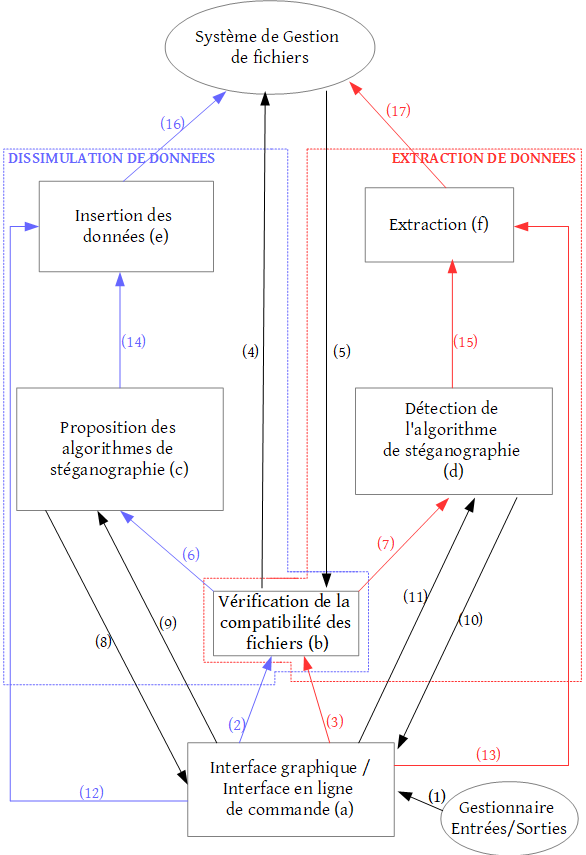
\includegraphics[scale=0.71]{pictures/organigramme.png}

\subsection{Liste des modules et de leurs fonctionnalités}

\begin{description}
\item[a)] \textbf{Interface graphique / Interface en ligne de commande} :
    interfaces permettant à l'utilisateur de choisir parmi les deux
    fonctionnalités possibles de l'application. Il peut dissimuler des
    données dans un fichier (dont le type et le format sont pris en charge
    par l'application). Ou bien, il peut extraire les données cachées d'un
    fichier. \newline
    Il aura donc un mécanisme pour choisir le fichier hôte et le fichier 
    à cacher (pour la dissimulation de données), et un mécanisme pour choisir le 
    fichier contenant les données cachées à analyser (pour l'extraction de 
    données cachées), grâce à une interaction avec le gestionnaire Entrée/Sorties. 

\item[b)] \textbf{Vérification de la compatibilité des fichiers} : le format 
	du fichier hôte (pour le module \textit{Dissimulation de données}) ou 
	le format du fichier à analyser (pour le module \textit{Extraction de données 
	cachées}), choisis par l'utilisateur, est vérifié pour savoir s'il est 
	bien pris en charge par l'application. \newline
	Il aura un mécanisme de lecture du fichier hôte : selon les formats 
	pris en charge, il y aura une batterie de tests pour déterminer le 
	format du fichier. 
	Il prendra en entrée les chemins de fichiers en entrée. Ce module interagira
	avec le gestionnaire de Gestion de Fichiers. 

\item[c)] \textbf{Proposition des algorithmes de stéganographie} : en fonction
    du type et du format du fichier hôte, ainsi que de la taille des données à
    cacher, un mécanisme proposera un ou plusieurs algorithmes (avec ou sans 
    sécurité supplémentaire). Si il y a un mot de passe, l'interface va 
    donner le mot de passe à ce module, ainsi que l'algorithme choisi. 

\item[d)] \textbf{Détection de l'algorithme de stéganographie} : un mécanisme 
	d'analyse du fichier permettra de découvrir quel algorithme a été utilisé 
	afin de les extraire correctement par la suite. S'il est nécessaire 
	d'utiliser un mot de passe pour déchiffrer les données cachées, le module 
	récupèrera le champ mot de passe de l'interface. 

\item[e)] \textbf{Insertion des données} : la copie des données du fichier hôte
    sera modifiée avec l'insertion des données à cacher à l'aide de l'algorithme
    choisi par l'utilisateur. 
    Il prendra en entrée le fichier à cacher, le fichier hôte, le chemin du 
    fichier résultant, l'algorithme à utiliser ainsi que le mot de passe 
    s'il y en a un. 

\item[f)] \textbf{Extraction} : les données cachées dans le fichier à analyser
    sont extraites. Les algorithmes utilisés pour l'insertion des données 
    et l'extraction seront expliqués dans la sous-section \textit{"Algorithmes 
    de dissimulation et d'extraction en stéganographie"}. 
    Ce module prendra en entrée le fichier à analyser, le chemin du fichier 
    à extraire et l'algorithme détecté. 

\end{description}

\newpage

\section{Description des structures de données}

\subsection{Description des énumérations}

\begin{lstlisting}[language=c]
enum mode {STEGX_MODE_INSERT, STEGX_MODE_EXTRACT};
typedef enum mode mode_e;
\end{lstlisting}

L'énumération mode permet de distinguer les deux outils proposés par 
l'application : extraire ou dissimuler. 
\newline

\begin{lstlisting}[language=c]
enum algo {STEGX_ALGO_LSB, STEGX_ALGO_EOF, STEGX_ALGO_METADATA};
typedef enum algo algo_e;
\end{lstlisting}

L'énumération algo distingue les différents algorithmes proposés par 
l'application. 
\newline 

\begin{lstlisting}[language=c]
enum type {BMP_COMPRESSED, BMP_UNCOMPRESSED, PNG, WAV_PCM, WAV_NO_PCM, 
        MP3, AVI_COMPRESSED, AVI_UNCOMPRESSED, FLV, UNKNOWN};
typedef enum type type_e;
\end{lstlisting}

L'énumération type expose les différents formats de fichiers avec leurs 
particularités pour certains. Si le format du fichier hôte ou à analyser 
est inconnu, cela sera représenté par le type UNKNOWN. \newline

\subsection{Description des types}

\subsection{Description des structures}

%\begin{lstlisting}[language=c]
%struct stegx_infos {
%    enum type type;
%    union{
%        stegx_bmp bmp;
%        stegx_png png;
%        stegx_wav wav;
%        stegx_mp3 mp3;
%        stegx_avi avi;
%        stegx_flv flv;
%    } infos;
%};
%typedef struct stegx_infos STEGX_INFOS;
%\end{lstlisting}

%Cette première structure stegx\_infos permet de stocker les informations 
%utiles pour chaque format différent afin de le manipuler convenablement 
%par la suite. 
%\newline
%\underline{Paramètres :}
%\begin{itemize}
%\item \textit{type} permet de distinguer quel champ il faut manipuler pour l'union 
%infos. Pour chaque format, il y un ou plusieurs types possibles.
%\item \textit{infos} est une union en C. Elle permet de choisir un champ parmi
%ceux qui sont définis. Ainsi, si le fichier hôte est un fichier BMP par exemple, 
%seul la structure bmp de infos sera initialisée et manipulée par la suite.
%\newline
%\end{itemize}

\begin{lstlisting}[language=c]
struct stegx_info_ins {
    char* hidden_path;
    algo_e algo;
};
typedef struct stegx_info_ins stegx_info_ins_s;
\end{lstlisting}

La structure stegx\_info\_ins permet de représenter les informations 
nécessaire sur le fichier à cacher, c'est-à-dire son chemin et l'algo que 
l'on utilisera pour dissimuler ce dernier. \newline
\underline{Paramètres :}
\begin{itemize}
\item \textit{hidden\_path} est une chaine de caractères représentant le nom du fichier 
à cacher. 
\item \textit{algo} représente l'algorithme qui sera utilisé pour dissimuler. 
\newline
\end{itemize}

\begin{lstlisting}[language=c]
struct stegx_info {
    char* host_path;
    char* res_path;                         
    char* passwd;                           
    mode_e mode;                            
    stegx_info_ins_s* ins_info;             
};
typedef struct stegx_info stegx_info_s;
\end{lstlisting}

La structure stegx\_info représente la structure publique (de la bibliothèque
de StegX). Elle représente les données choisies par l'utilisateur s'il veut 
dissimuler ou extraire des données. \newline
\underline{Paramètres :}
\begin{itemize}
\item \textit{host\_path} est une chaine de caractères représentant le chemin
du fichier à analyser (pour l'extraction) ou hôte (pour la dissimulation). 
\item \textit{res\_path} est une chaine de caractères représentant le chemin
du fichier résultant (pour l'extraction ou pour la dissimulation). 
\item \textit{passwd} est une chaine de caractères représentant le mot de passe 
choisi par l'utilisateur. Celui-ci est optionnel et si l'utilisateur choisit 
de ne pas en mettre, passwd vaudra NULL. 
\item \textit{mode} est une variable d'énumération représentant le mode que 
l'utilisateur a choisi : dissimulation (STEGX\_MODE\_INSERT)ou extraction 
(STEGX\_MODE\_EXTRACT). 
\item \textit{* ins\_info} est un pointeur sur la structure stockant les informations 
sur le fichier à cacher. Elle est requise si le champ mode est à STEGX\_MODE\_INSERT. 
\newline
\end{itemize}

\begin{lstlisting}[language=c]
struct host_info {
    FILE* host;
    type_e type;
    union {
        struct bmp bmp;
        struct png png;
        struct wav wav;
        struct mp3 mp3;
        struct avi avi;
        struct flv flv;
    } file_type;
};
typedef struct host_info host_info_s;
\end{lstlisting}

Cette structure stegx\_infos permet de stocker les informations 
utiles pour chaque format différent afin de le manipuler convenablement 
par la suite. 
\newline
\underline{Paramètres :}
\begin{itemize}
\item \textit{host} représente le fichier hôte pour le cas de la dissimulation 
et le fichier à analyser pour le cas de l'extraction. 
\item \textit{type} permet de distinguer quel champ il faut manipuler pour l'union 
infos. Pour chaque format, il y un ou plusieurs types possibles.
\item \textit{infos} est une union en C. Elle permet de choisir un champ parmi
ceux qui sont définis. Ainsi, si le fichier hôte est un fichier BMP par exemple, 
seule la structure bmp de infos sera initialisée et manipulée par la suite.
\newline
\end{itemize}

\begin{lstlisting}[language=c]
struct info {
    mode_e mode;                
    host_info_s host;           
    FILE* res;                 
    FILE* hidden;              
    char* hidden_name;
    int hidden_length; 
    char* passwd;
    algo_e algo;
};
typedef struct info info_s;
\end{lstlisting}

La structure info\_s correspond à la structure privée de la bibliothèque. 
Elle va contenir toutes les informations utiles pour la dissimulation ou 
l'extraction des données. 
\newline
\underline{Paramètres :}
\begin{itemize}
\item \textit{mode} est une variable d'énumération représentant le mode que 
l'utilisateur a choisi : dissimulation (STEGX\_MODE\_INSERT)ou extraction 
(STEGX\_MODE\_EXTRACT). 
\item \textit{host} va contenir le détail du fichier hôte pour le bon déroulement 
de la dissimulation/extraction (selon les cas d'utilisation). 
\item \textit{res} représente le fichier résultat qui va être créé pour la 
dissimulation ou l'extraction.  
\item \textit{hidden} représente le fichier à cacher dans le cas de l'insertion. 
Il est donc requis si mode vaut STEGX\_MODE\_INSERT. 
\item \textit{hidden\_name} représente le nom du fichier à cacher/caché selon 
les cas. 
\item \textit{hidden\_length} représente la taille du fichier à cacher/caché. 
Cette information est nécessaire dans l'extraction pour connaitre combien de 
données il reste à extraire dans le fichier. Dans la dissimulation, ce champ 
permet de construire correctement les informations globales du fichier caché. 
\item \textit{passwd} est la chaine de caractères représentant le mot de passe 
choisi par l'utilisateur. 
\item \textit{algo} est l'énumération représentant l'algorithme qui sera utilisé
pour la dissimulation ou l'extraction. 
\newline
\end{itemize}

\section{Description des fonctions des différents modules}

\subsection{Module Interface graphique}

Pour l'interface graphique, on utilisera la librairie GTK+. Pour l'implémentation 
de l'interface graphique, il faudra donc étudier quels widgets utilisés 
ainsi que les signaux pour mettre en relation ces derniers avec les 
actions de l'utilisateur. 

L'interface permettra à l'utilisateur de manipuler correctement l'application 
StegX. Ainsi, un utilisateur, non adepte à l'informatique, réussira à 
utiliser l'application. 
Pour réaliser cette interface, nous allons créé une structure nommée 
\textit{struct ui} qui va correspondre à l'interface utilisateur. Cette 
structure va notamment contenir tous les widgets utilisés dans l'interface 
utilisateur. 

\begin{lstlisting}[language=c]
void ui_create (GtkWidget* window, struct ui* ui);
\end{lstlisting}

Cette fonction va permettre de créer entièrement l'interface utilisateur 
sur une fenêtre donnée. Elle construira les widgets et configure les signaux. 
\newline
\underline{Entrées :} 
\begin{itemize}
\item \textit{*window :} pointeur vers la fenêtre sur laquelle construire 
l'interface utilisateur. 
\item \textit{*ui :} pointeur vers l'interface utilisateur à remplir. 
\newline 
\end{itemize}

\begin{lstlisting}[language=c]
void ui_delete (struct ui* ui);
\end{lstlisting}

Cette fonction va supprimer l'interface utilisateur. Elle permettra de 
désallouer la mémoire utilisée pour l'interface utilisateur. 
\newline
\underline{Entrée :} 
\begin{itemize}
\item \textit{*ui :} pointeur vers l'interface utilisateur à désallouer. 
\newline 
\end{itemize}

\begin{lstlisting}[language=c]
void ui_build (struct ui* ui);
\end{lstlisting}

Cette fonction va construire la fenêtre principale en ajoutant les conteneurs 
et les widgets. 
\newline
\underline{Entrée :} 
\begin{itemize}
\item \textit{*ui :} pointeur vers l'interface utilisateur où il faut construire 
l'affichage. 
\newline 
\end{itemize}

\begin{lstlisting}[language=c]
void ui_signal_init (struct ui* ui);
\end{lstlisting}

Cette fonction va initialiser les signaux et connecter ces derniers aux 
widgets de la fenêtre principale. 
\newline
\underline{Entrée :} 
\begin{itemize}
\item \textit{*ui :} pointeur vers l'interface utilisateur où il faut 
configurer les signaux. 
\newline 
\end{itemize}

La structure \textit{struct ui} et les 4 fonctions sont les outils principaux 
pour construire l'interface graphique. Ainsi, cela permet de visualiser 
en amont le fonctionnement de l'interface graphique de StegX. 

\subsection{Module Interface en ligne de commande}

Concernant l'interface en ligne de commande, c'est le deuxième moyen pour 
manipuler l'application StegX. Les utilisateurs savant manipuler le terminal 
peuvent ainsi faire de la stéganographie. 

\begin{lstlisting}[language=c]
stegx_info_s* init_stegx_info ();
\end{lstlisting}

Cette fonction va initialiser la structure contenant les informations 
entrées en ligne de commande. 
\newline
\underline{Sortie :} 
\begin{itemize}
\item \textit{stegx\_info\_s:} renvoie la structure initialisée. 
\newline 
\end{itemize}

\begin{lstlisting}[language=c]
void fill_info (stegx_info_s* com, const int argc, char* const* argv);
\end{lstlisting}

La fonction va remplir la structure avec les informations entrées en 
ligne de commande. 
\newline
\underline{Entrée :} 
\begin{itemize}
\item \textit{*com :} pointeur sur la structure contenant les informations 
entrées par l'utilisateur. 
\item \textit{argc :} nombre d'arguments entrés en ligne de commande. 
\item \textit{argv :} arguments entrés en ligne de commande. 
\newline 
\end{itemize}

\begin{lstlisting}[language=c]
void we_are_stegx ();
\end{lstlisting}

Cette fonction va afficher la présentation du projet. \newline

\begin{lstlisting}[language=c]
void help ();
\end{lstlisting}

La fonction \textit{help} va afficher l'aide du lancement de l'application 
en ligne de commande et détaille les différents paramètres à spécifier 
pour l'utilisateur. \newline

\begin{lstlisting}[language=c]
void unvalid_line (stegx_info_s* com);
\end{lstlisting}

Cette fonction avertira l'utilisateur d'une erreur lors du lancement 
de l'application en ligne de commande et affiche l'aide. \newline

\underline{Entrée :} 
\begin{itemize}
\item \textit{*com :} pointeur sur la structure contenant les informations 
entrées par l'utilisateur. 
\newline 
\end{itemize}

\begin{lstlisting}[language=c]
void check_info (stegx_info_s* com);
\end{lstlisting}

Cette fonction vérifiera les informations entrées par l'utilisateur et 
que l'utilisateur a bien indiqué les informations nécessaires pour 
la dissimulation ou l'extraction. \newline

\underline{Entrée :} 
\begin{itemize}
\item \textit{*com :} pointeur sur la structure contenant les informations 
entrées par l'utilisateur. 
\newline 
\end{itemize}

\begin{lstlisting}[language=c]
void dest_stegx_info (stegx_info_s* com);
\end{lstlisting}

Cette fonction va libérer la structure contenant les informations entrées 
en ligne de commande. \newline

\underline{Entrée :} 
\begin{itemize}
\item \textit{*com :} pointeur sur la structure contenant les informations 
entrées par l'utilisateur. 
\newline 
\end{itemize}

\subsection{Module Vérification de la compatibilité des fichiers}

D'après l'organigramme créé lors du cahier des charges, ce module prend en 
entrée les chemins du fichier hôte et du fichier à cacher (pour la dissimulation) ; 
le chemin du fichier à analyser (pour l'extraction). Il va interagir avec 
le système de fichiers pour pouvoir vérifier la compatibilité des fichiers en entrée. 
Enfin, après sa vérification, ce module va envoyer les fichiers aux modules 
\textit{Proposition des algorithmes de stéganographie} (pour dissimuler) ou 
\textit{Détection de l'algorithme de stéganographie} (pour extraire). 
Ainsi, cette communication se fera à l'aide de la structure privée de la 
bibliothèque \textit{info\_s}. 
\newline

\begin{lstlisting}[language=c]
info_s* stegx_check_compatibility_dissimulation (stegx_info_s* infos);
\end{lstlisting}

Cette fonction analyse la compatibilité des fichiers hôte et à cacher pour
la dissimulation. Ces données sont dans la structure info mis en paramètre. 
Pour cela, elle vérifie que les fichier hôte et à cacher existent et qu'ils 
ne sont pas vides. Ensuite, la fonction vérifie le format du fichier hôte. 
Elle va remplir les champs \textit{mode}, \textit{passwd}, \textit{hidden\_name}, \textit{hidden},
\textit{res} et \textit{host} (partiellement) de la structure
\textit{info\_s*} en sortie. 
\newline
\underline{Entrée :}
\begin{itemize}
\item \textit{*infos :} structure publique que les interfaces vont initialiser.
\end{itemize}
\underline{Sortie :}
\begin{itemize}
\item \textit{info\_s* :} pointeur sur une structure initialisée 
partiellement pour insérer les informations nécessaires à la vérification 
de la compatibilité des fichiers en entrée. 
\newline 
\end{itemize}

\begin{lstlisting}[language=c]
info_s* stegx_check_compatibility_extraction (stegx_info_s* infos);
\end{lstlisting}

Cette fonction analyse la compatibilité du fichier à analyser pour l'extraction. 
Pour cela, elle vérifie si le fichier à analyser existe et n'est pas vide. 
Ensuite, la fonction vérifie le format du fichier à analyser. 
Elle va remplir les champs \textit{mode}, \textit{hidden\_name}, \textit{hidden},
\textit{res} et \textit{host} (partiellement) de la structure
\textit{info\_s*} en sortie. 
\newline
\underline{Entrée :}
\begin{itemize}
\item \textit{*infos :} structure publique que les interfaces vont initialiser.
\end{itemize}
\underline{Sortie :}
\begin{itemize}
\item \textit{info\_s* :} pointeur sur une structure initialisée 
partiellement pour insérer les informations nécessaires à la vérification 
de la compatibilité des fichiers en entrée. 
\newline 
\end{itemize}

\begin{lstlisting}[language=c]
int stegx_test_file_not_empty (FILE* file);
\end{lstlisting}

Cette fonction teste si le fichier n'est pas vide. 
\newline
\underline{Entrée :}
\begin{itemize}
\item \textit{file :} fichier à tester.
\end{itemize}
\underline{Sortie :} 
\begin{itemize}
\item \textit{int :} renvoie 0 si le fichier est vide ou qu'il n'existe pas ; 1 sinon. 
\newline \end{itemize}

\begin{lstlisting}[language=c]
type_e stegx_test_file_bmp (FILE* file);
type_e stegx_test_file_png (FILE* file);
type_e stegx_test_file_wav (FILE* file);
type_e stegx_test_file_mp3 (FILE* file);
type_e stegx_test_file_avi (FILE* file);
type_e stegx_test_file_flv (FILE* file);
\end{lstlisting}

Ces fonctions testent le format du fichier en lisant le fichier en entrée 
(Magic Number notamment). 
\newline
\underline{Entrée :} 
\begin{itemize}
\item \textit{file :} fichier à tester. 
\end{itemize}
\underline{Sortie :} 
\begin{itemize}
\item \textit{type\_e :} renvoie UNKNOWN si le format du fichier n'est pas pris en 
charge par l'application ; sinon, en fonction du format et des particularités 
du fichier, il peut renvoyer \textit{BMP\_COMPRESSED}, \textit{BMP\_UNCOMPRESSED}, 
\textit{PNG}, \textit{WAV\_PCM}, \textit{MP3}, \textit{AVI\_COMPRESSED}, 
\textit{AVI\_UNCOMPRESSED} ou \textit{FLV}. 
\newline 
\end{itemize}

\begin{lstlisting}[language=c]
type_e check_file_format (FILE* file);
\end{lstlisting}

Cette fonction récupère le fichier dont le format est à trouver. Elle établit une 
batterie de tests pour déterminer si le format du fichier est pris en charge 
par l'application. 
Pour cela, on utilisera les fonctions 
$type\_e$ $stegx\_test\_file\_XXX (FILE* file)$ comme vu précedemment. 
\newline
\underline{Entrée :} 
\begin{itemize}
\item \textit{file :} fichier à tester. 
\end{itemize}
\underline{Sortie :} 
\begin{itemize}
\item \textit{type\_e :} renvoie UNKNOWN si le format du fichier n'est pas pris en 
charge par l'application ; sinon, en fonction du format et des particularités 
du fichier, il peut renvoyer \textit{BMP\_COMPRESSED}, \textit{BMP\_UNCOMPRESSED}, 
\textit{PNG}, \textit{WAV\_PCM}, \textit{MP3}, \textit{AVI\_COMPRESSED}, 
\textit{AVI\_UNCOMPRESSED} ou \textit{FLV}. 
\newline 
\end{itemize}

\subsection{Module Proposition des algorithmes 
de stéganographie}

Dans l'organigramme des modules de StegX, nous avons créé un sous-module 
\textit{Proposition des algorithmes de stéganographie}. Il prend en entrée 
le fichier hôte, le fichier à cacher, le choix de l'utilisateur pour 
l'algorithme ainsi que le mot de passe voulu par l'utilisateur. 
Ce sous-module va donc ajouter des données à la structure \textit{info\_s} 
avec notamment l'algorithme de stéganographie utilisé choisi à partir de ceux 
proposés. 

\begin{lstlisting}[language=c]
void* stegx_suggest_algo_stegano (info_s* infos, stegx_info_s* user_choices);
\end{lstlisting}

Cette fonction va remplir les champs \textit{passwd} et \textit{host.file\_type} 
de \textit{info} pour le sous-module suivant \textit{insertion des données}. 
De plus, elle va changer les valeurs du tableau représentant les algorithmes 
de stéganographie utilisés. Ainsi, à partir de ce tableau, l'interface graphique 
proposera certains algorithmes, et l'interface en ligne de commande comparera 
ce tableau avec le choix de l'utilisateur. 
\newline
\underline{Entrées :} 
\begin{itemize}
\item \textit{infos :} structure représentant toutes les informations pour 
réaliser l'insertion par la suite. 
\item \textit{user\_choices :} structure représentant les choix de 
l'utilisateur pour les deux interfaces. 
\end{itemize}
\underline{Sortie :} 
\begin{itemize}
\item \textit{void* :} renvoie NULL si tout se passe bien. [a remodifier 
comme definition]. 
\newline 
\end{itemize}

\begin{lstlisting}[language=c]
int fill_host_file_type (info_s* infos);
\end{lstlisting}

En fonction du champ \textit{infos.host.type} représentant le format du 
fichier hôte, cette fonction va remplir le champ \textit{host.file\_type} 
de \textit{infos}. En effet, \textit{file\_type} est une union et est 
particulière en fonction du format du fichier hôte. 
\newline
\underline{Entrée :} 
\begin{itemize}
\item \textit{infos :} structure représentant toutes les informations pour 
l'insertion. 
\end{itemize}
\underline{Sortie :} 
\begin{itemize}
\item \textit{int :} renvoie 0 si il y a une erreur détectée dans cette 
fonction et 1 si tout se passe bien. 
\newline 
\end{itemize}

\begin{lstlisting}[language=c]
int can_use_algo_lsb (info_s* infos);
int can_use_algo_eof (info_s* infos);
int can_use_algo_metadata (info_s* infos);
\end{lstlisting}

Ces fonctions vont permettre de savoir si les différents algorithmes 
(LSB, EOF, Metadata) peuvent être utilisés en fonction des entrées 
de l'utilisateur à travers l'interface (graphique ou en ligne de commande). 
\newline
\underline{Entrée :} 
\begin{itemize}
\item \textit{infos :} structure représentant toutes les informations pour 
l'insertion.  
\end{itemize}
\underline{Sortie :} 
\begin{itemize}
\item \textit{int :} renvoie 0 si le fichier hôte ne peut pas cacher des 
données selon l'algorithme, et 1 s'il le peut. 
\newline 
\end{itemize}

\begin{lstlisting}[language=c]
int stegx_choose_algo_stegano (info_s* infos, stegx_infos_s* user_choices); 
\end{lstlisting}

A partir du champ \textit{ins\_info.algo} de la structure \textit{user\_choices}, 
ainsi que du tableau représentant les algorithmes utilisables (selon les 
entrées de l'utilisateur), cette fonction change le champ \textit{algo} 
\textit{infos}. 
\newline
\underline{Entrées :} 
\begin{itemize}
\item \textit{infos :} structure représentant toutes les informations pour 
l'insertion.  
\item \textit{user\_choices :} structure représentant les choix de 
l'utilisateur pour les deux interfaces. 
\end{itemize}
\underline{Sortie :} 
\begin{itemize}
\item \textit{int :} renvoie 0 si il y a une erreur détectée dans cette 
fonction et 1 si tout se passe bien.  
\newline 
\end{itemize}

\subsection{Module Détection de l'algorithme de
stéganographie}

Le sous-module \textit{Détection de l'algorithme de stéganographie} prend en 
entrée le fichier à analyser. De plus, il récupère grâce à l'interface le 
mot de passe choisi par l'utilisateur.  
Ce sous-module va compléter les champs des structures \textit{info\_s} 
et \textit{stegx\_info\_s} avec en particulier l'algorithme de stéganographie 
utilisé par l'émetteur et que l'application doit détecter pour extraire 
correctement les données cachées. 

\begin{lstlisting}[language=c]
int stegx_read_signature_app (info_s* infos, stegx_info_s user_choices); 
\end{lstlisting}

Cette fonction va lire la signature insérée dans le fichier à analyser. 
Cette signature est constituée d'un octet représentant quel algorithme a 
été utilisé, avec le nom et la taille du fichier caché.  
\newline
\underline{Entrées :} 
\begin{itemize}
\item \textit{infos :} structure représentant toutes les informations pour 
l'extraction.  
\item \textit{user\_choices :} structure représentant les choix de 
l'utilisateur. 
\end{itemize}
\underline{Sortie :} 
\begin{itemize}
\item \textit{int :} renvoie 0 si il y a une erreur détectée dans cette 
fonction et 1 si tout se passe bien.  
\newline 
\end{itemize}

\begin{lstlisting}[language=c]
void* detect_algo_stegano (info_s* infos, stegx_info_s* user_choices); 
\end{lstlisting}

Cette fonction va tout d'abord récupérer le mot de passe choisi par 
l'utilisateur et initialisé le champ \textit{infos.passwd}. Ensuite, à 
l'aide de la fonction \textit{fill\_host\_file\_type}, le champ-union 
\textit{infos.host.file\_type} sera initialisé. Enfin, cette fonction appellera 
\textit{stegx\_read\_signature\_app} pour connaître les informations concernant 
le fichier caché. 
\newline
\underline{Entrées :} 
\begin{itemize}
\item \textit{infos :} structure représentant toutes les informations pour 
l'extraction.  
\item \textit{user\_choices :} structure représentant les choix de 
l'utilisateur. 
\end{itemize}
\underline{Sortie :} 
\begin{itemize}
\item \textit{void* :} renvoie NULL si tout se passe bien. [a remodifier 
comme definition]. 
\newline 
\end{itemize}

\subsection{Module Insertion des données}
\subsection{Module Extraction}

\section{Conclusion}


\end{document}
